\documentclass{article}

\usepackage{graphicx}
\usepackage{graphpap}
\usepackage{amsmath}
\usepackage{fancyhdr}



%%%%%%%%%%%%%%%%%%%%%%%%%%%%%%%%%%%%%%%%5
%
%  Set Up Margins

%%%%%%%%%%%%%%%%%%%%%%%%%%%%%%%%%%%%%%%%%%%%%%%%%
% include file for:
%      Critical Page setup dimensions
%            DO NOT MODIFY
%       (for help see "Latex Line by Line" p 260)
%
\setlength\oddsidemargin{0in}
\setlength\evensidemargin{0in}

\usepackage[left=0.98in, right=0.98in, top=1.0in, bottom=1.0in]{geometry}

% %Top Margin and header
% \setlength\voffset{-0.94in}
% \setlength\topmargin{0.25in}
% \setlength\headheight{0.25in}
% %\setlength\headwidth{6.5in}
% \setlength\headsep{0.25in}
% %Body
% \setlength\textwidth{6.5in}
% \setlength\textheight{9.50in}
% %Footer
% %\setlength\footheight{0.5in}
% \setlength\footskip{0.3750in}
% Line spacing for 6 lines per inch
\linespread{0.894}  % 1.0 = single    1.6 = double
%
%          END of Critical Page Setup Dimensions
%%%%%%%%%%%%%%%%%%%%%%%%%%%%%%%%%%%%%%%%%%%%%%%%%%%

%%%%%%%%%%%%%%%%%%%%%%%%%%%%%%%%%%%%%%%%%%%%%%%%%%%
%
% Useful style and math macros
%


\newcommand\Dfrac[2]{\frac{\displaystyle #1}{\displaystyle #2}}
\newcommand\beq{\begin{equation}}
\newcommand\eeq{\end{equation}}

\newcommand\bmat{\begin{bmatrix}}
\newcommand\emat{\end{bmatrix}}

\newenvironment{solution}
{\vspace{0.125in} {\bf SOLUTION:} \\ }
{\vspace{0.25in}}



%%%%%%%%%%%%%%%%%%%%%%%%%%%%%%%%%%%%%%%%%%%%%%%%%
%
%         Page format Mods HERE
%
%Mod's to page size for this document
\addtolength\textwidth{0cm}
\addtolength\oddsidemargin{0cm}
\addtolength\headsep{0cm}
\addtolength\textheight{0cm}
%\linespread{0.894}   % 0.894 = 6 lines per inch, 1 = "single",  1.6 = "double"

%%%%%%%%%%%%%%%%%%%%%%%%%%%%% HEADER / FOOTER
\pagestyle{fancy}
%%%%%  Page header/footer fields for "NSF Style" proposal
%%%%%  \chead will be changed with each section
\lhead{\small\sc EE543}
\rhead{Wtr 2018}
\chead{Problem Set 1}
\lfoot{Hannaford, U. of Washington}
\rfoot{\today}
\cfoot{\thepage}
%\renewcommand\headrulewidth{1pt}
%\renewcommand\footrulewidth{1pt}

\begin{document}

%%%%** Section 1
\section{Problem Set 1}

%%%%** Section 1.1
\subsection{Rotation Matrix}
Two frames are superimposed as shown below

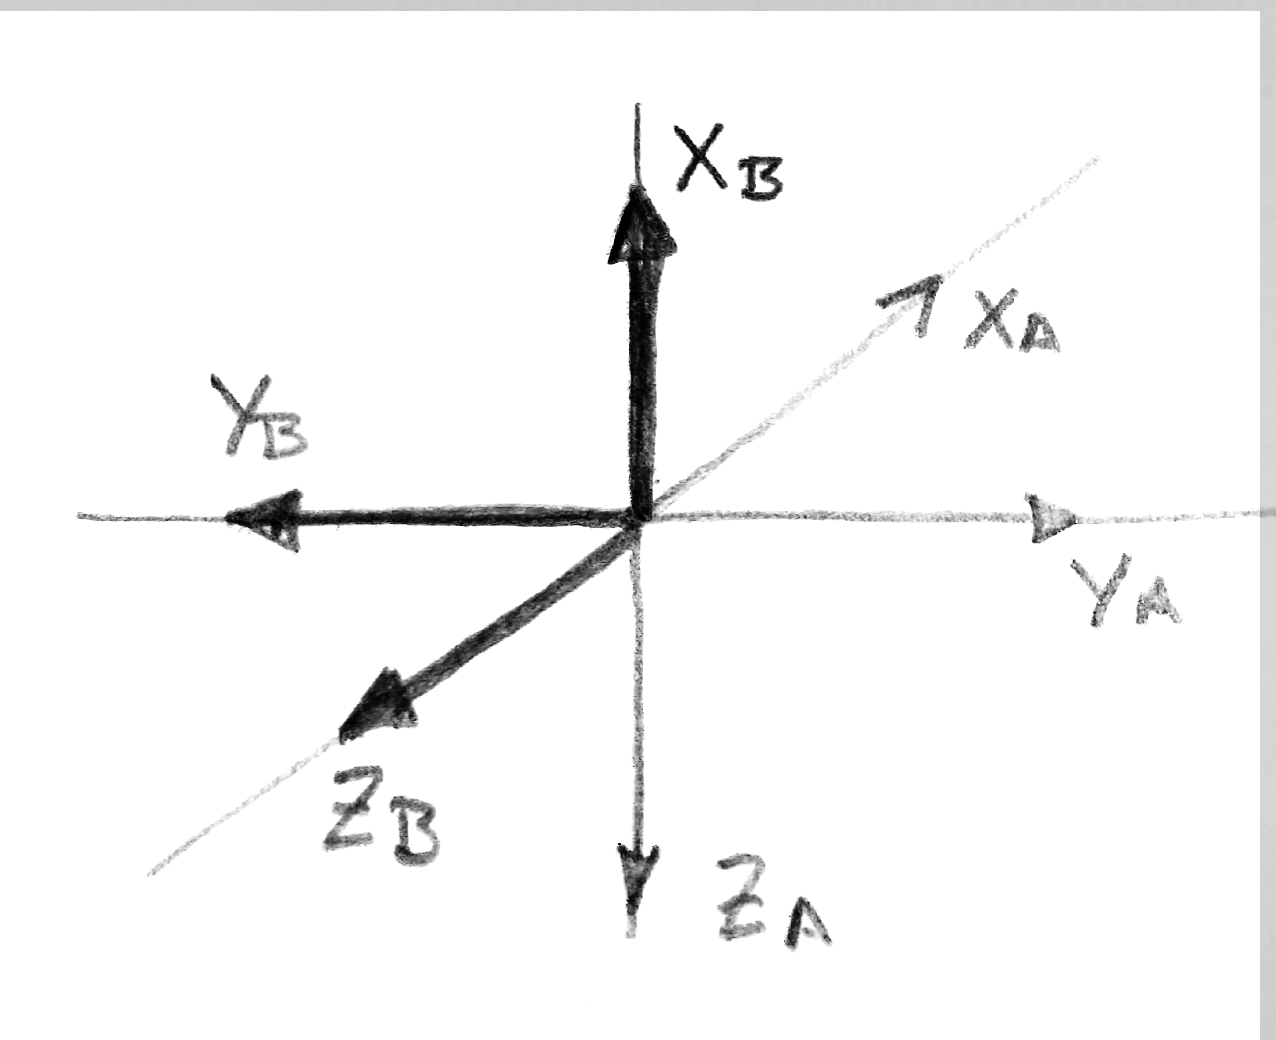
\includegraphics[width=1.5in]{hw1p1_w18.png}

Give the rotation matrix, $^A_BR$


%%%%** Section 1.2
\subsection{Composition of Rotations}
Two frames, $A, B$ start out superimposed.

1) Frame $B$ is rotated by $\alpha$ around $Y_A$


2) Frame $B$ is rotated by $\beta$ around $X_A$


3) Frame $B$ is rotated by $\gamma$ around $Y_B$

Find $^A_BR$


%%%%** Section 1.3
\subsection{Composition of Rotations}
Two frames, $A, B$ start out superimposed.

1) Frame $B$ is rotated by $45^\circ$ around $Y_B$


2) Frame $B$ is rotated by $119^\circ$ around $Z_A$


3) Frame $B$ is rotated by $16^\circ$ around $Z_B$

Find $^A_BR$
 



%%%%** Section 1.4
\subsection{Composition of Rotations}
Two frames, $A, B$ start out superimposed.

1) Frame $B$ is rotated by $27.5^\circ$ around $X_B$


2) Frame $B$ is rotated by $-37.5^\circ$ around $Z_A$


3) Frame $B$ is rotated by $126^\circ$ around $Z_B$

Find $^A_BR$. Multiply out your answer in numerical form.





%%%%** Section 1.5
\subsection{Angle-Axis Rotation}
Using the result of Section 2.4 and 2.6 (see notes), show that if $K=\bmat 1 & 0 & 0 \emat ^T$ then
\[
Rot(K,\theta) = Rot(\hat{x}, \theta)
\]


%%%%** Section 1.6
\subsection{Composition of Rotations and RPY}

The following rotations are performed

\begin{enumerate}
  \item A roll-pitch-yaw rotation in which

   Roll = $16^\circ$, Pitch = $5^\circ$, Yaw = $4^\circ$

  \item A rotation about the current $Y$ axis by $45^\circ$.
  \item A rotation about the original $X$ (Roll) axis by $20^\circ$.
\end{enumerate}

Find the rotation matrix which represents the final orientation.   Multiply out your answer in numerical form.

\end{document}

